\input{"C:/Users/spileggi/Google Drive/STAT 330/Lectures/SlideStyle.tex"}



\title[Lecture 8]{Arrays and DO loops}
\author[Pileggi]{Shannon Pileggi}

\institute[STAT 330]{STAT 330}

\date{}


\begin{document}

\begin{frame}
\titlepage
\end{frame}

\begin{frame}
\frametitle{OUTLINE\qquad\qquad\qquad} \tableofcontents[hideallsubsections]
\end{frame}



%===========================================================================================================================
\section[DO loops]{DO loops}
%===========================================================================================================================
\subsection{}
\begin{frame}
\ft{Overview}
\bi
\item \ttt{DO} loops can be used to perform a series of statements on an observation any number of times
\item they can be handy when creating a data set from scratch or calculating something that happens at regular intervals (ex. annual interest rates)
\item Some details:
\bi
\item \ttt{DO} loops always need to end with the statement \fbox{\ttt{END;}}
\item There is an implicit \emph{output} at the end of each data step.  If you want to create an observation for each iteration, place \fbox{\ttt{OUTPUT;}} inside the \ttt{DO} loop.
\ei
\ei
\end{frame}

\begin{frame}[fragile]
\ft{OUTPUT statement}
SAS uses an \ttb{implicit} \ttt{output} statement at the \ttb{end} of the data step \ttb{only} if the data step does not contain the word \ttt{output}.  The two codes below are equivalent:
\vskip10pt
\footnotesize
\bmp{0.5\textwidth}
\footnotesize
\begin{code}{.0}
DATA example1 ;
    DO i = 1 TO 4 ;
    END ;
RUN ;

\end{code}
\emp
\bmp{0.05\textwidth}
\hspace*{0.05in}
\emp
\bmp{0.5\textwidth}
\footnotesize
\begin{code}{.0}
DATA example2 ;
    DO i = 1 TO 4 ;
    END ;
    \textcolor{OrangeRed}{OUTPUT ;}
RUN ;
\end{code}
\emp
\end{frame}


\begin{frame}[fragile]
\ft{OUTPUT statement}
The default position for the \ttb{implicit} \ttt{output} statement always right before the \texttt{RUN;} statement - but we can move it!
\vskip10pt
\footnotesize

\bmp{0.45\textwidth}
\footnotesize
\begin{code}{.0}
DATA example2 ;
    DO i = 1 TO 4 ;
    END ;
    \textcolor{OrangeRed}{OUTPUT ;}
RUN ;
\end{code}
\begin{center}
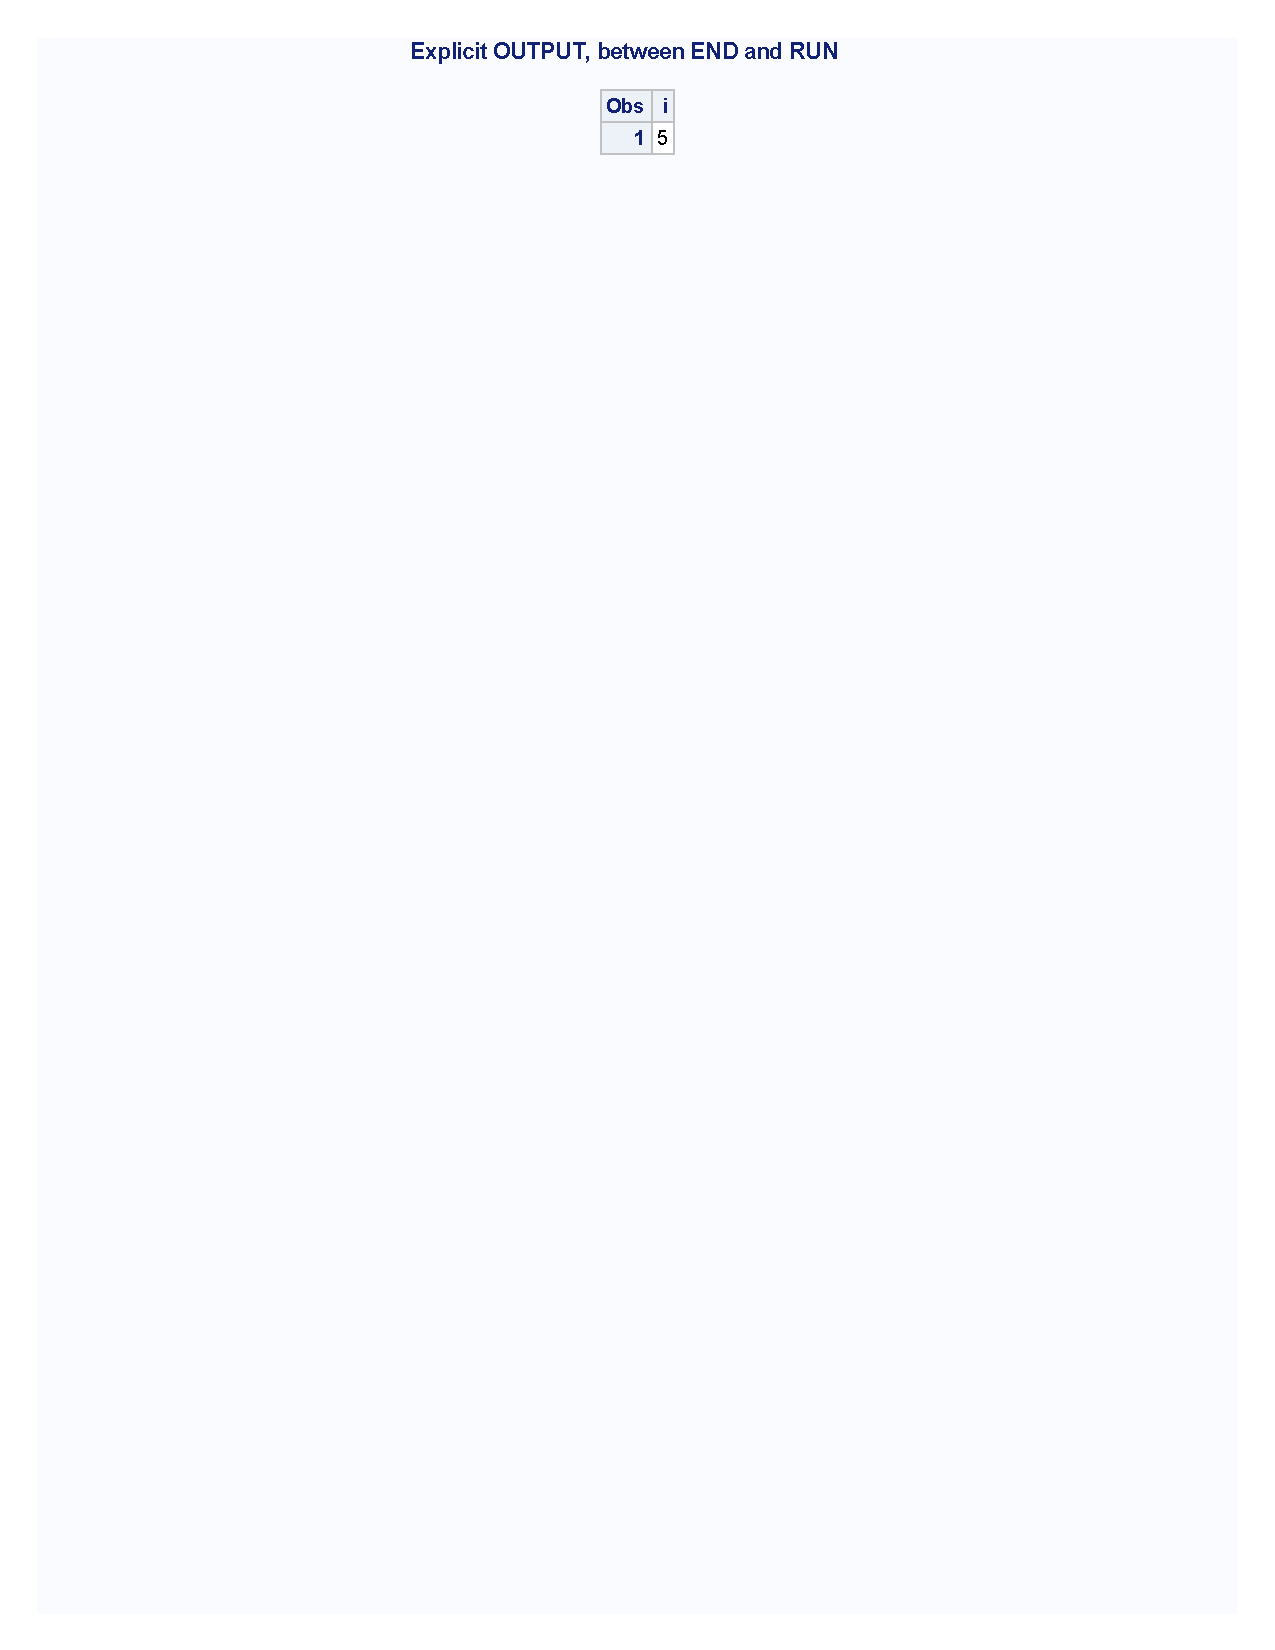
\includegraphics[trim=10cm 23cm 10cm 1.5cm,clip,width=0.30\textwidth]{L8_ex2.pdf}
\end{center}
\emp
\bmp{0.05\textwidth}\hspace{1in}\emp
\bmp{0.45\textwidth}
\begin{code}{.0}
DATA example3 ;
    DO i = 1 TO 4 ;
        \textcolor{OrangeRed}{OUTPUT ;}
    END ;
RUN ;
\end{code}
\begin{center}
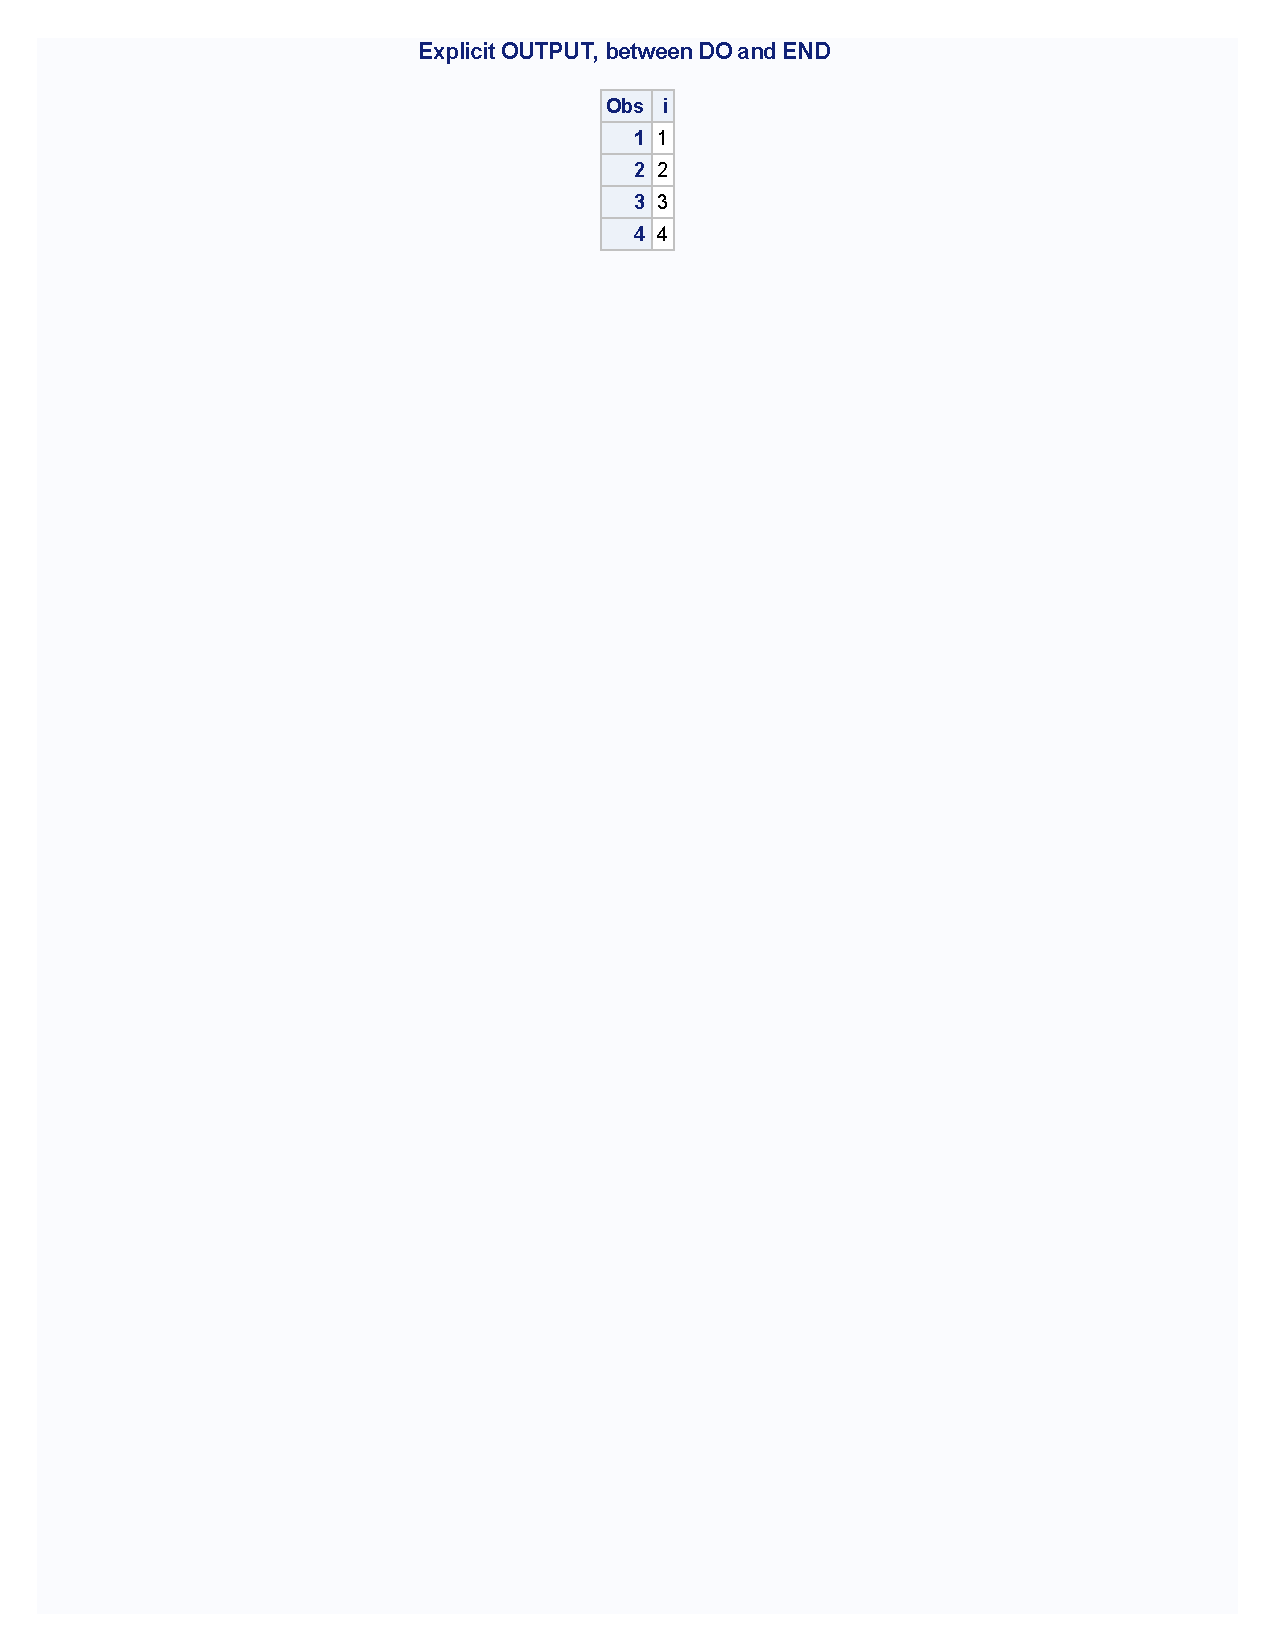
\includegraphics[trim=10cm 23cm 10cm 1.5cm,clip,width=0.30\textwidth]{L8_ex3.pdf}
\end{center}
\emp
\end{frame}


\begin{frame}
\ft{Index variables}
\bi
\item In the previous example, we used \ttt{i} as the \emph{index} variable.
\item Index variables don't have to be used in the inner \texttt{DO/END} block, but SAS does keep track of its values.
\item By default, SAS will increase the index variable by $+1$
\item The index variable is increased by the default value at the \emph{bottom} of each loop iteration when SAS encounters the \fbox{\ttt{END;}} statement.
\item So, at the termination of the loop, the value of the index variable is one increment beyond the stop value.
\ei
\end{frame}



\begin{frame}[fragile]
\fto
How could you modify the \texttt{example3} code to show each iteration of \emph{i} and the last value of \emph{i}?
\vskip10pt
\footnotesize
\bmp{0.45\textwidth}
\footnotesize
\begin{code}{.0}
DATA example2 ;
    DO i = 1 TO 4 ;
    END ;
    \textcolor{OrangeRed}{OUTPUT ;}
RUN ;
\end{code}
\begin{center}
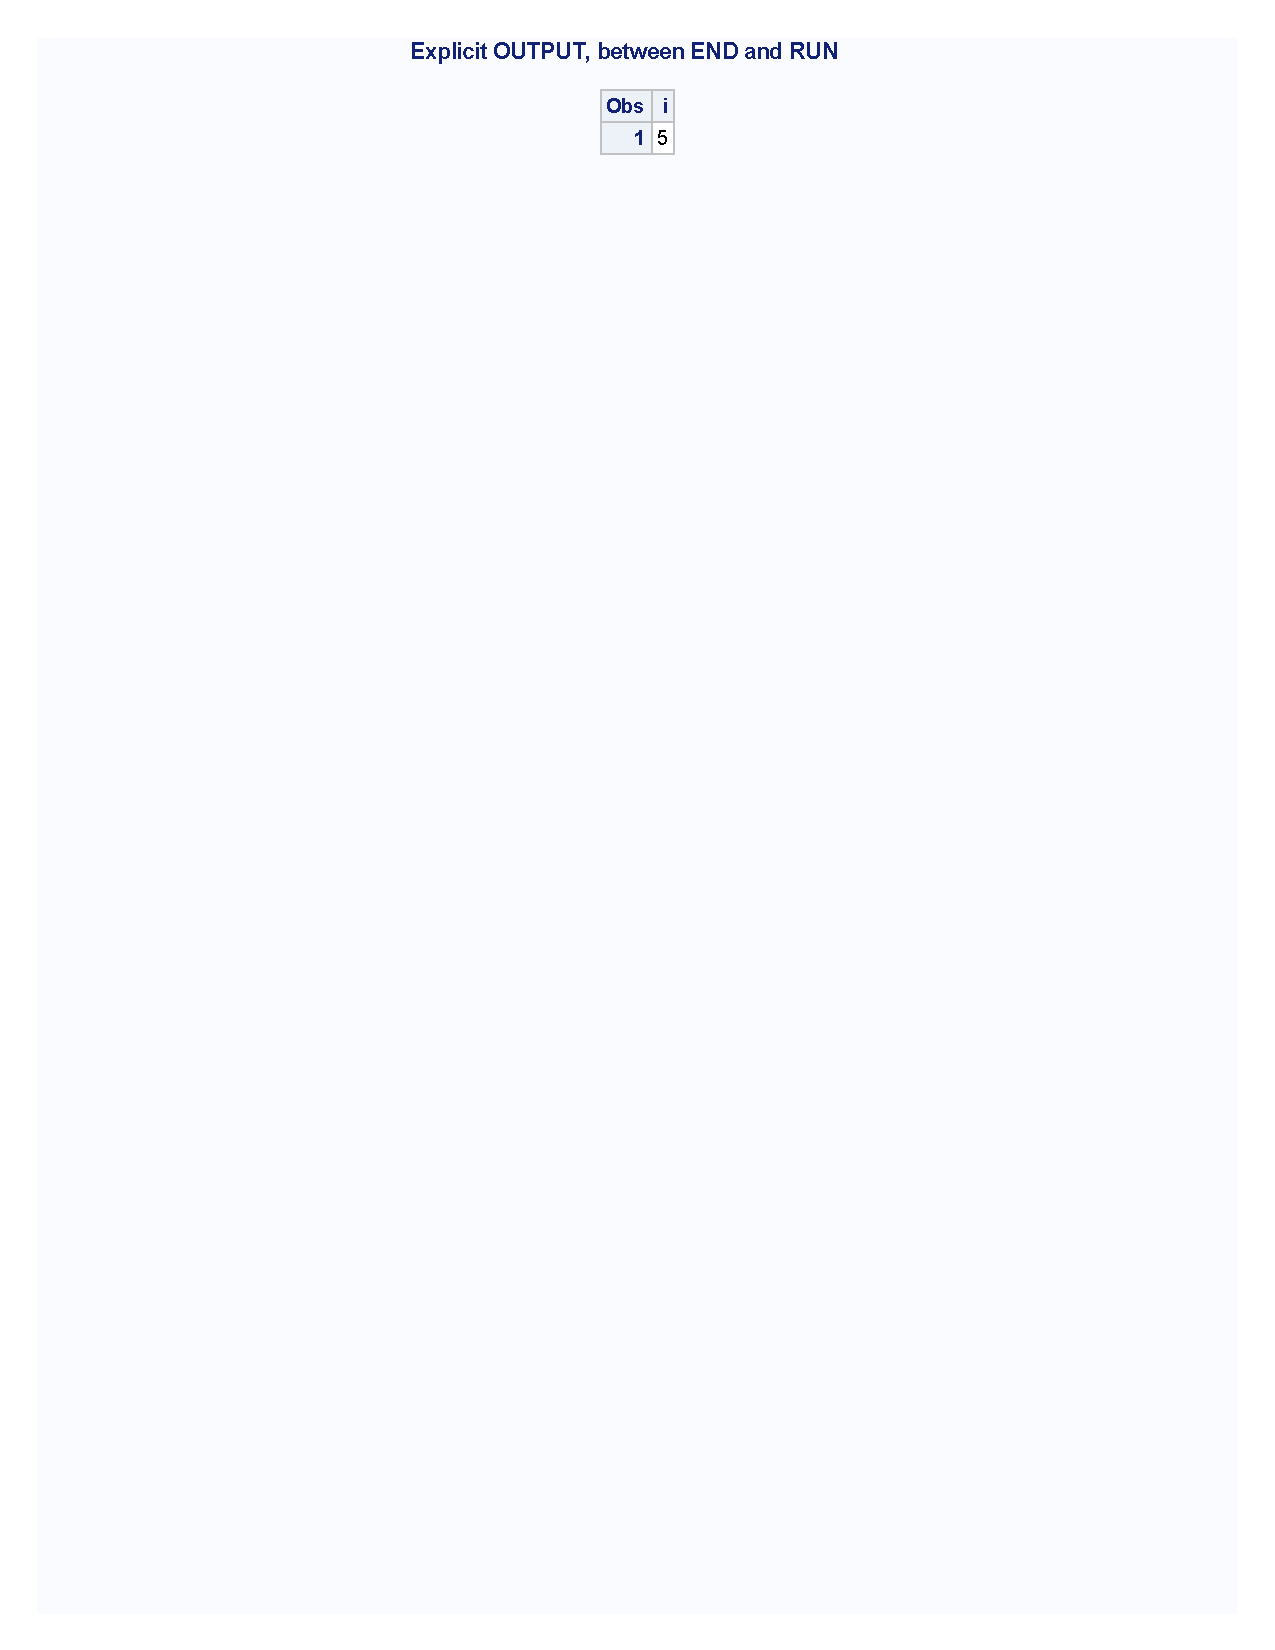
\includegraphics[trim=10cm 23cm 10cm 1.5cm,clip,width=0.30\textwidth]{L8_ex2.pdf}
\end{center}
\emp
\bmp{0.05\textwidth}\hspace{1in}\emp
\bmp{0.45\textwidth}
\begin{code}{.0}
DATA example3 ;
    DO i = 1 TO 4 ;
        \textcolor{OrangeRed}{OUTPUT ;}
    END ;
RUN ;
\end{code}
\begin{center}
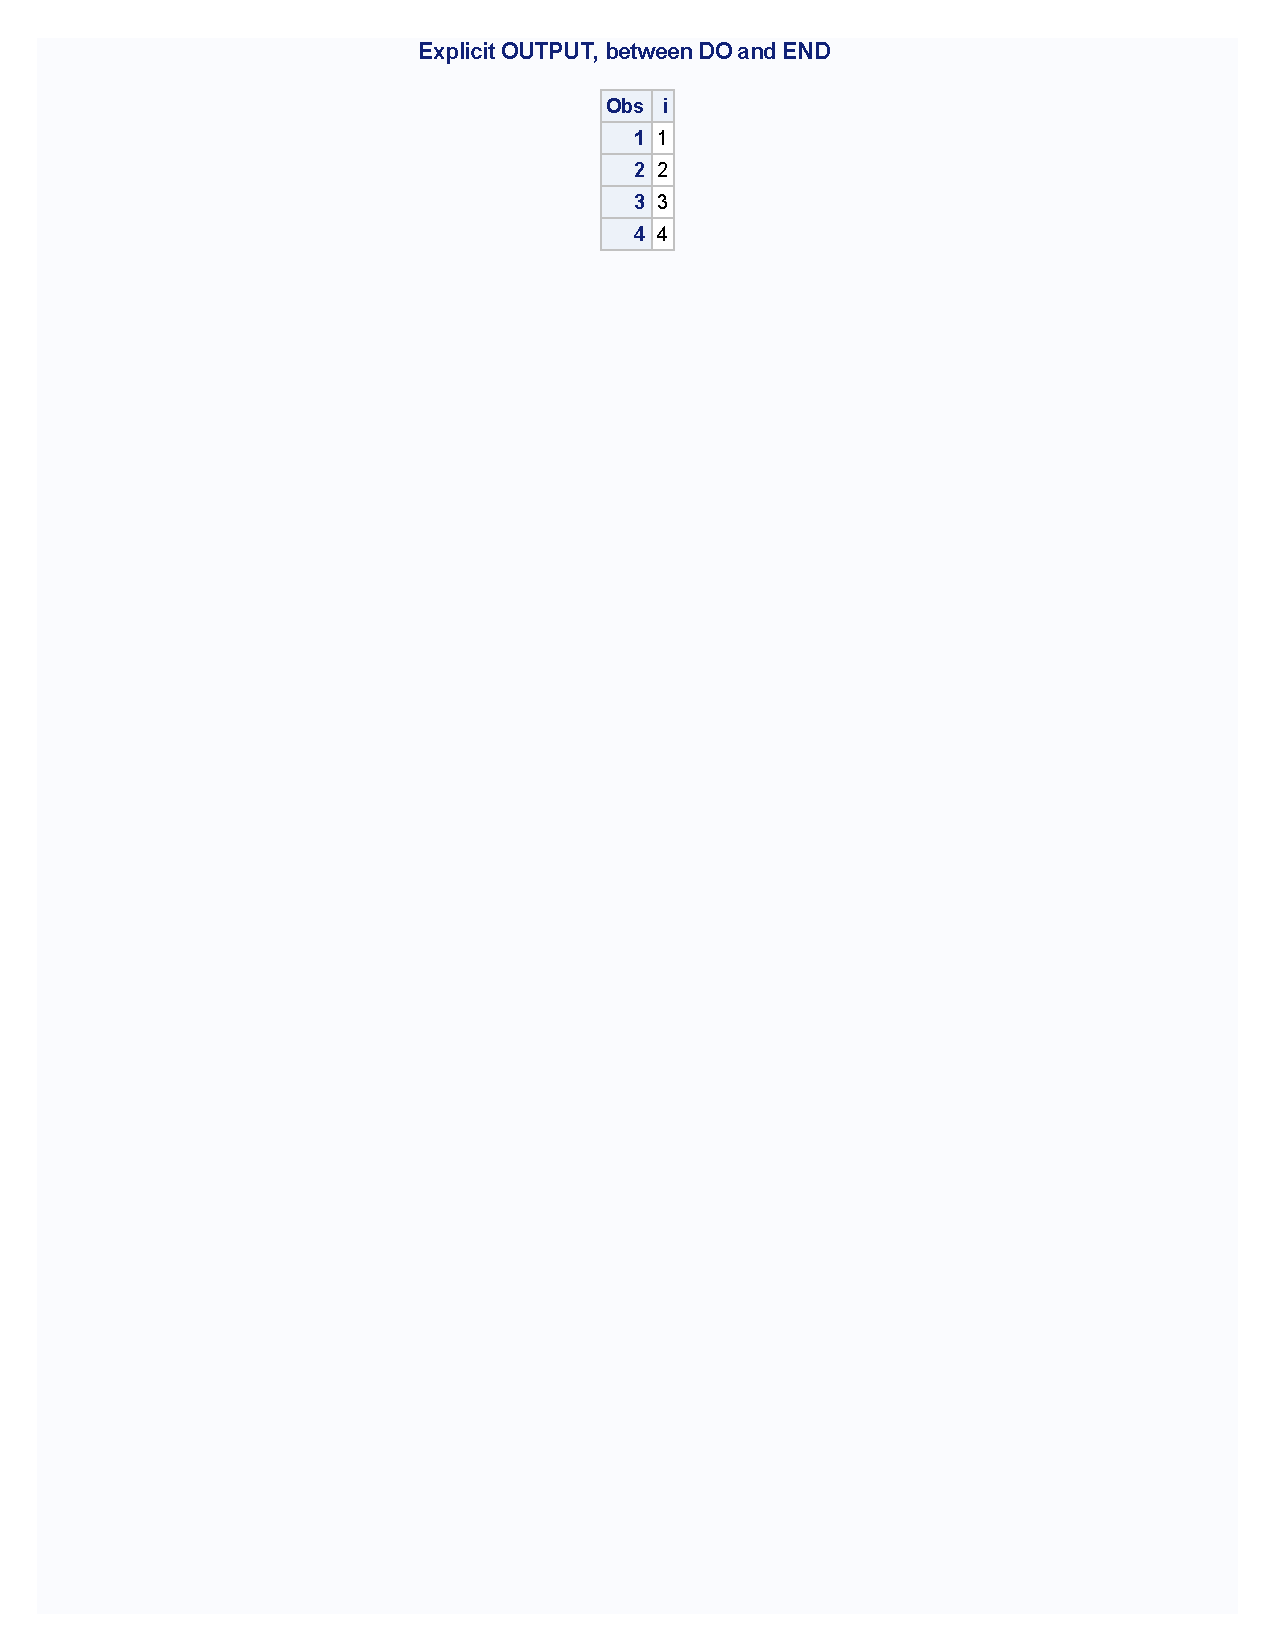
\includegraphics[trim=10cm 23cm 10cm 1.5cm,clip,width=0.30\textwidth]{L8_ex3.pdf}
\end{center}
\emp
\end{frame}

\begin{frame}
\ft{Changing the Loop Increment/Decrement Method}
\begin{tabular}{ll}
\ttt{do i=0 to 10 by 2;} & \ttt{i=0,2,4,6,8,10}\\
[1ex]
\ttt{do j=1 to 10 by 2;} & \ttt{j=1,3,5,7,9}\\
[1ex]
\ttt{do k=1 to 10 by .1;} & \ttt{k=1,1.1,1.2,...,9.9,10}\\
[1ex]
\ttt{do l=10 to 1 by -1;} & \ttt{l=10,9,8,...,1}	\\
[1ex]
\ttt{do m=2,6,9,11,22;} & \ttt{specify nonstandard index values}\\
[1ex]
\ttt{do n="A","B","C";} & \ttt{specify character index values}	\\
[1ex]
\ttt{do o=var1,var2,var3;} & \ttt{specify variables}	\\
\end{tabular}
\end{frame}

\begin{frame}
\begin{clicker}{What are the final values of the index variables?}
\begin{enumerate}[A.]
    \item \ttt{DO i = 1 TO 5; ... END;}
    % final value = 6
    \item \ttt{DO j = 2 TO 8 by 2; ... END;}
    % final value = 10
    \item \ttt{DO k = 10 TO 2 by -2;  ... END;}
    % final value = 0
\end{enumerate}
\end{clicker}
\end{frame}

\begin{frame}[fragile]
\ft{Nested do loops}
\bmp{.5\textwidth}
\footnotesize
\begin{code}{.0}
DATA example5 ;
   DO i = 1 TO 3;
      DO j = "A","B" ;
         x + 1 ;
         OUTPUT ;
      END ;
   END ;
RUN ;

\end{code}
\normalsize
\emp
\ \hspace{.4in} \
\bmp{.3\textwidth}
\bt{|ccc|} \hline
\multicolumn{3}{|c|}{Variables Table}\\
\multicolumn{3}{|c|}{for DO Loop}\\ \hline
 \ttt{i}  &  \ttt{j}  & \quad  \ttt{x} \quad \\ \hline 	
1 & A & 1 \\
1 & B & 2\\
2 & A & 3\\
2 & B & 4\\
3 & A & 5\\
3 & B & 6\\
\hline
\et
\emp
\vskip10pt
\oyo Predict the output that you would see if you moved the \ttt{OUTPUT} statement to after the first \fbox{\ttt{END;}}.
\end{frame}


%===========================================================================================================================
\section[DO UNTIL/WHILE]{DO UNTIL/WHILE}
%===========================================================================================================================
\subsection{}
\begin{frame}
\tableofcontents[currentsection, hideallsubsections]
\end{frame}

\begin{frame}
\ft{Modified \ttt{DO} Loop: DO UNTIL}

\bi
\item \ttt{DO UNTIL} is a special loop that \ttb{breaks} the iteration process when a \tte{condition} is met
\item \ttb{SAS Syntax:} \ttt{DO UNTIL (\tte{condition});}
\item Helpful when the number of iterations is not known ahead of time
\item \ttb{Important note:} SAS checks on the status of the condition \ttb{at the bottom} of the loop (when it encounters the \ttt{END;} statement).
\item[]
\ei
\begin{clicker}{Which of the following is TRUE?}
\begin{enumerate}
\item A \ttt{DO UNTIL} loop always executes at least once %TRUE!
\item A \ttt{DO UNTIL} may never execute %FALSE!
\end{enumerate}
\end{clicker}
\end{frame}

\begin{frame}
\ft{Modified \ttt{Do} Loop: DO WHILE}
\bi
\item \ttt{DO WHILE} is a special loop that \ttb{continues} the iteration process as long as  a \tte{condition} is met
\item \ttb{SAS Syntax:} \ttt{do while (\tte{condition});}
\item Helpful when the number of iterations is not known ahead of time
\item \ttb{Important note:} SAS checks on the status of the condition \ttb{at the start} of the loop.
\item[]
\ei
\begin{clicker}{Which of the following is TRUE?}
\begin{enumerate}
\item A \ttt{DO WHILE} loop always executes at least once %FALSE!
\item A \ttt{DO WHILE} may never execute %TRUE!
\end{enumerate}
\end{clicker}
\end{frame}

\begin{frame}[fragile]
\ft{Example Code}
\hspace*{-0.2in}
\bmp{0.25\textwidth}
Suppose my annual income is \$60,000, and I expect it to increase by 2\% every year, and I plan to save 10\% of my annual income each year.  How many years until I save \$500,000?
\emp
\bmp{0.05\textwidth}
\hspace*{0.05in}
\emp
\bmp{0.80\textwidth}
\footnotesize
\begin{code}{.0}
DATA retire ;
	savings = 0 ;
	income = 60000 ;
	year = 0 ;

	DO UNTIL (savings >= 500000) ;
    /*----------------------------*/
    /*    WORKS EQUIVALENTLY      */
    /*DO WHILE (savings < 500000);*/
    /*----------------------------*/
		year = year + 1 ;
		savings = savings + income*.10 ;
		income = income + income*.02 ;
		OUTPUT ;
	END ;
RUN ;
\end{code}
\emp
\end{frame}


\begin{frame}[fragile]
\fto
\bmp{0.40\textwidth}
\footnotesize
\begin{code}{.0}
DATA example6 ;
   x = 15 ;
   DO WHILE(x > 12) ;
      x + 1 ;
   END ;
RUN ;
\end{code}
\emp
\bmp{0.05\textwidth}
\hspace*{0.05in}
\emp
\bmp{0.50\textwidth}
\begin{clicker}{What is the value of \emph{x} at the completion of this \ttt{DATA} step?}
\begin{enumerate}
    \item 12
    \item 15
    \item 16
    \item this loop executes infinitely %CORRECT!!
\end{enumerate}
\end{clicker}
\emp
\end{frame}

\begin{frame}[fragile]
\fto
\bmp{0.5\textwidth}
\footnotesize
\begin{code}{.0}
DATA example7 ;
   x = 0 ;
   \textcolor{OrangeRed}{/*ENTER LINE HERE*/}
      x = x + 1 ;
      x_sq = x**2 ;
      OUTPUT ;
   END ;
RUN ;
\end{code}
\emp
\bmp{0.05\textwidth}
\hspace*{0.05in}
\emp
\bmp{0.5\textwidth}
\begin{clicker}{Suppose I wanted to generate the sequence of numbers $1^2, 2^2, 3^2, 4^2$.  Which line of code would achieve this?}
\begin{enumerate}
\item \ttt{DO UNTIL(x < 4);}
\item \ttt{DO WHILE (x < 4);} %THIS ONE
\item \ttt{DO UNTIL(x = 5);}
\item \ttt{DO WHILE (x = 5);}
\end{enumerate}
\end{clicker}
\emp
\end{frame}

%===========================================================================================================================
\section[Arrays]{Arrays}
%===========================================================================================================================
\subsection{}
\begin{frame}
\tableofcontents[currentsection, hideallsubsections]
\end{frame}

\begin{frame}[fragile]
\ft{Data}
\bmp{1.0\textwidth}
\footnotesize
\begin{code}{.0}
DATA grades;
   INPUT name $ exam1 exam2 exam3;
   DATALINES;
   Shannon      96    82    83
   Lex          92    81    68
   Becky        92    75    73
   Lora         94    65    70
   Susan        91    77    85
   Hunter       76    72    86
   Ulric        98    71    80
   Richann      90    60    60
   Tim          97    94   100
   Ronald        .    77    60
   ;
RUN;
\end{code}
\emp
\end{frame}

\begin{frame}[fragile]
\ft{Motivating Example}
An \emph{inefficient} way to convert all test scores to letter grades:
\bmp{1.0\textwidth}
\footnotesize
\begin{code}{.0}
DATA grades2 ;
	SET grades ;
	*FOR EXAM1;
	IF exam1 = . THEN letter1 = " " ;
	ELSE IF exam1 <60 THEN letter1 = "F";
	ELSE IF 60 <= exam1 < 70 THEN letter1 = "D";
	ELSE IF 70 <= exam1 < 80 THEN letter1 = "C";
	ELSE IF 80 <= exam1 < 90 THEN letter1 = "B";
	ELSE IF 90 <= exam1 THEN letter1 = "A";
	/*Repeat code chunk for exam2*/
	/*Repeat code chunk for exam3*/
RUN ;
\end{code}
\emp
\end{frame}

\begin{frame}
\ft{About arrays}
\bi
\item \ttb{Purpose of SAS Arrays:}  An array is a temporary grouping of variables under a \ttb{single name}.
\bi
\item must be all character or all numeric
\item can be existing variables or new variables that you would like to create
\ei
\item Helps reduce the number of required statements to process variables
\item Can simplify the maintenance of DATA step programs
\item NOTE: Arrays only exist during the data step, although the variables they work with may be a part of the data set.
\ei
\end{frame}

\begin{frame}
\ft{Defining an Array}
\bi
%\item To group previously defined data set variables into an array, use an \ttt{ARRAY} statement that specifies
%\bi
%	\item the array's name
%	\item its dimension/size enclosed in braces, brackets, or parentheses
%	\item the elements to associate with the array members
%\ei	
\item \ttb{SAS Syntax:}  \ttt{ARRAY  \tte{array\_name} \tte(dimension)  \tte{elements};}
\item The name of the array must not be a SAS keyword or an existing variable
\item[] \fbox{\ttt{array scores (3) exam1 exam2 exam3 ;}}
\item The array \ttt{scores} contains the variables \ttt{exam1}, \ttt{exam2}, and \ttt{exam3}.
\item To reference a variable using an array call the array name and then the appropriate subscript,
\item[]i. e., \ttt{scores(2)} refers to \ttt{exam2}
\ei
\end{frame}

\begin{frame}[fragile]
\ft{Example code}
An \emph{efficient} way to convert all test scores to letter grades:
\bmp{1.0\textwidth}
\footnotesize
\begin{code}{.0}
DATA grades2 ;
   SET grades ;

   ARRAY scores (*) exam: ;

   ARRAY letters (3) $ ;

   DO i = 1 TO DIM(SCORES) ;
      IF scores(i) = . THEN letters(i) = " " ;
      ELSE IF scores(i) <60 THEN letters(i) = "F";
      ELSE IF 60 <= scores(i) < 70 THEN letters(i) = "D";
      ELSE IF 70 <= scores(i) < 80 THEN letters(i) = "C";
      ELSE IF 80 <= scores(i) < 90 THEN letters(i) = "B";
      ELSE IF 90 <= scores(i) THEN letters(i) = "A";
   END ;
RUN ;
\end{code}
\emp
\end{frame}

\begin{frame}
\ft{Shortcuts for listing variables}
\bi
\item Numbered range lists are for variables that start with the same characters and end with consecutive numbering
    \bi
    \item \ttt{Var6 Var7 Var8} is the same as \ttt{Var6-Var8}
    \ei
\item Name range lists depend on the position of the variables in the data set
    \bi
    \item \ttt{Cat Cow Pig Dog} is the same as \ttt{Cat -- Dog}
    \item[](Assuming that this is the position order in the data set)
    \item How can you check the order?  Use \ttt{PROC contents}!
    \ei
\item You can use these shortcuts inside of functions
    \bi
    \item e.g., \ttt{X = mean(of Var1-Var5)}
    \ei
\item When variables have the same prefix, you can also call all variables with that prefix
    \bi
    \item e.g., \ttt{Y = sum(of Var:)}
    \ei
\ei
\end{frame}


\begin{frame}[fragile]
\begin{center}
\fbox{\ttt{array assignments (\textcolor{OrangeRed}{?}) hw1 hw2 hw3 hw4;}}
\end{center}
\vskip10pt
\begin{clicker}{What belongs within the parentheses of this \ttt{array} statement?}
\begin{enumerate}
\item \ttt{hoemwork}
\item \ttt{homework*}
\item \ttt{1-4}
\item \ttt{4}
\end{enumerate}
\end{clicker}
\end{frame}

\begin{frame}[fragile]
\ft{A more complex array}
\bmp{1.0\textwidth}
\footnotesize
\begin{code}{.0}
DATA grades2 ;
   SET grades ;

   ARRAY scores (*) exam: ;

   ARRAY letters (3) $ ;

   ARRAY letter_values (6) $ (" " "F" "D" "C" "B" "A");

   ARRAY grcuts (6) (0 60 70 80 90 100);

   DO i = 1 TO DIM(SCORES) ;
		
   DO j = 2 to 6 ;
       IF grcuts(j-1) <= scores(i) <= grcuts(j)
       THEN letters(i) = letter_values(j) ;
   END ;
   END ;
RUN ;
\end{code}
\emp
\end{frame}



\end{document} 